\chapter{Generative Adversarial Networks : Principles, strengths and limitations}
\label{chap:chapter1}

\begin{chapterabstract}
	In this chapter, we first propose an introduction to the problem of generative modeling and some solutions to tackle this problem. We then propose an overview of the Generative Adversarial Networks \cite{Goodfellow2014} framework, which is a recent method to train deep neural networks as generative models that is particularly adapted to the task of image generation. We will introduce some of its theoretical interpretations, as well as some of its variations and applications. We discuss the different limitations of this approach and expose a trilemma between the quality of the generated samples, their diversity and the conditioning of the model. We then discuss the recent advances that have been made to overcome some of these limitations and propose a taxonomy of these advances using the aforementioned trilemma. Finally, we discuss the evaluation of generative models and the difficulties of evaluating the intrinsic quality of a generated sample.  We propose an overview of the different classical metrics and discuss their limitations.
\end{chapterabstract}

\minitoc
\newpage

\section{Generative modeling}
we will first propose an overview of generative modeling

Generative modeling with deep neural networks has been a challenging task due to the stochastic nature of sampling, which prevents the computation of gradient, thus preventing the training of a deep model with gradient descent.  \CR{TODO}%TODO

\subsection{Generative modeling with maximum likelihood estimation}

\begin{figure}
	\centering
	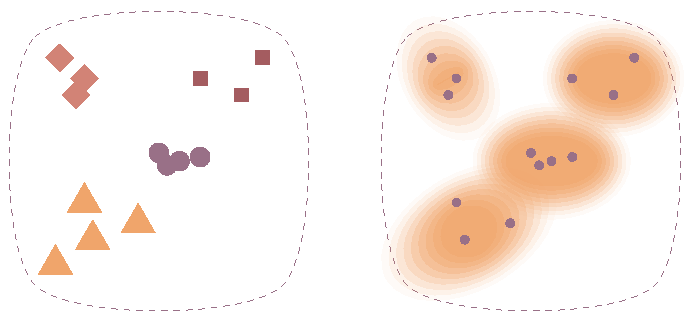
\includegraphics[height=\textheight/3,width=\textwidth]{chapter1/disc_gen}
	\caption[Generative modeling]{Left: Discriminative modeling, the model aims to find decision boundaries between classes. Right: Generative modeling, the model aims to learn the probability distribution of the data.}
	\label{fig:disc_gen}
\end{figure}

Generative modeling is the task of learning the underlying distribution of a dataset in order to generate more samples from that distribution. In other words, it describes how data is generated in terms of a probabilistic model,  a distribution from which the whole dataset could have been sampled with a high likelihood.

 Indeed,  whereas a discriminative model tries to find decision boundaries by fitting a parametric model $\pt{\vy|\vx}$  to a conditional probability distribution $\p{\vy|\vx}$ of labels $\vy \in \setY$ relatively to the data $\vx \sim \p{x}$, a generative model aims to fit $\pt{\vx}$ to $\p{\vx}$  the intrinsic distribution of the data and to provide a sampling mechanism on this distribution (\seefigure{fig:disc_gen}).

These two learning tasks, the discriminative (\citeq{eq:disc_mle}) modeling and the generative modeling (\ \citeq{eq:gen_mle}) can be formulated as a maximum log-likelihood estimation\cite{Fisher1912}\\

\noindent\begin{minipage}{.5\linewidth}
	\begin{equation}
		\label{eq:disc_mle}
		\theta^* = \arg\max_\theta \esp{\vx,\vy\sim\p{y|x}} \log\pt{\vy|\vx}
	\end{equation}
\end{minipage}%
\begin{minipage}{.5\linewidth}
	\begin{equation}
			\label{eq:gen_mle}
		\theta^* = \arg\max_\theta \esp{\vx\sim\p{\vx}} \log\pt{\vx}
	\end{equation}
\end{minipage}\\

An simple example of generative model are Gaussian Mixture Models (\ac{GMM}) . They consist in a sum of $K$ Gaussian distributions $\mathcal{N}(\mu_k, \sigma_k^2), k \in 1..K$ which are all attributed a selection probability $p(z=k) = \pi_k$, so that 	$\p{\vx|z=k} = \mathcal{N}(\mu_k, \sigma_k^2)$ . The model is then formulated as 

\begin{equation*}
	\pt{\vx} = \sum_{z}\p{z}\pt{\vx|z}\enspace,
\end{equation*}

with log-likelihood 

\begin{equation*}
	\log\sum_{\vx\sim\p{\vx}}\pt{x}  = \sum_{\vx\sim\p{\vx}}\log\sum_{k=1}^k \pi_k \mathcal{N}(\vx|\mu_k, \sigma_k^2)\enspace.
\end{equation*}

In the case of the \ac{GMM}s, the Expectation-Maximization (\ac{EM}) algorithm \cite{Dempster1977} can be used to find the parameters $\theta^*$ which, at convergence, maximizes the log-likelihood of the model. Once the model is trained, sampling a new data is done by picking a component $k$ from the distribution $\p{z}$, then drawing a sample from the Gaussian distribution $\p{\vx|z=k} = \mathcal{N}(\mu_k^*, \sigma_k^{*2})$.

\subsection{Latent variable models}

\subsubsection{Latent variable models and marginalization}
For \ac{GMM}s, sampling a new point consists in, once the Gaussian component has been selected, sampling a point on a normal distribution.  This sampling can be done by using reparametrization: instead directly sampling $\vx \sim \mathcal{N}(\mu_k^*, \sigma_k^{*2})$, we can instead sample a latent variable $\vz \sim \mathcal{N}(0, 1)$ and compute $\vx = \G(\vz; \mu, \sigma) = \mu + \vz\sigma$.  Such a model, that consists in a deterministic function $\G: \setZ \rightarrow\setX$ with parameters $\theta$ applied to a random latent variable drawn from a fixed distribution $\p{\vz}$ is a latent variable model.

\begin{figure}
	\centering
	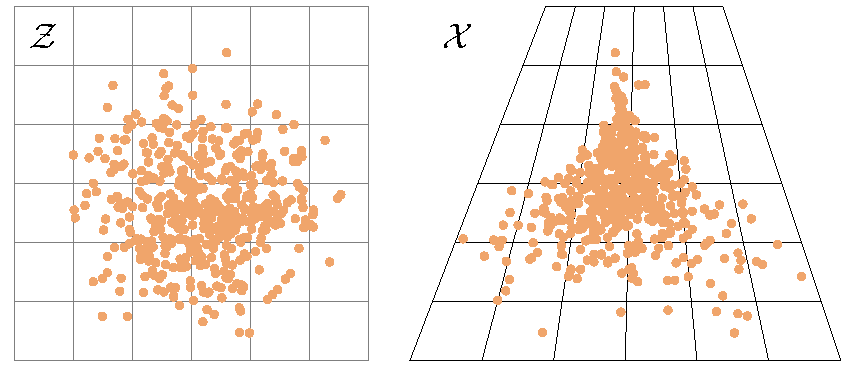
\includegraphics[height=\textheight/3,width=\textwidth]{chapter1/latent_model}
	\caption[Latent variable model]{A mapping between a latent space $\setZ$ and the space of a dataset $\setX$.}
\end{figure}

Since more complex distributions does not necessarily provide a natural sampling mechanism, using a latent variable model allows to outsource the stochastic part of the sampling  process from the learning process and only learn the function $\G(\vz; \theta)$. More formally, instead of directly modeling $\p{\vx}$, a latent variable model learns a deterministic mapping $\pg{\vx|\vz}$. From this mapping, the generative model can be obtain through marginalization 

\begin{equation}
	\pg{\vx} = \int_\setZ \p{\vz} \pg{\vx|\vz} d\vz = \int_\setZ \p{\vz} \p{\vx | G(\vz;\theta)} d\vz \enspace .
\end{equation}

This marginalization allows for the use of an arbitrary flexible $\G$. However, if $\G$ is non-linear, the actual evaluation of $\pg{\vx}$ is very likely to be intractable due to the integral over $\setZ$, which prevents the training of such a model as is.

While the marginal distribution $\pg{\vx}$ cannot be explicitly computed for any function $\G$, several solutions exist to overcome this problem and train deep generative models with latent variables anyways.  

\subsubsection{Variational auto-encoders}
\label{sub:deep_gen_modeling}

Variational Auto-Encoders (\ac{VAE})\cite{Kingmaa}  are deep latent variable models which tackle the marginalization problem by approximating the integral using a variational approach. To this end, they both learn the distribution of the latent model $\pg{\vx | \vz}$ as well as the distribution $\qf{\vz|\vx}$. This is done with  with two different neural networks, a decoder network  $\G:\setZ\rightarrow\setX$   and an encoder network $\F: \setX\rightarrow\setZ$ and allows to compute the distribution $\p{\vx}$ as

\begin{equation*}
	\log\pg{x} -  \DKL{\qf{\vz|\vx}}{\p{\vz|\vx}} = \esp{\vz\sim\qf{\vz|\vx}}\big[\log\pg{\vx|\vz}\big] - \DKL{\qf{\vz\vx}}{\p{\vz}}  \enspace .
\end{equation*}

The KL terms evaluates the distance between the distribution $\qf{\vz|\vx}$ learned by the encoder and real distribution $\p{\vz|\vx}$, and since $\p{\vz}$ is chosen Gaussian, this KL terms can be explicitly computed. The first term, is equivalent to the reconstruction error of an auto-encoder. Hence the model is trained by minimizing 

\begin{equation*}
	L_{VAE}(\F, \G) = \esp{\vz \sim \qf{\vz|\vx}}\big[ ||x - \G(\vz)||^2_2 \big] - \DKL{\qf{\vz|\vx}}{\p{\vz}}
\end{equation*}

However, since sampling $\vz \sim\qf{\vz|\vx}$ is not differentiable, the \ac{VAE} uses the so-called \textit{reparametrization trick}, that is to have $\F(\vx)$ output the mean and the variance $(\mu_\vx, \sigma^2_\vx)$ of a normal distribution for a sample $\vx$, so that a $\vz' \sim  \mathcal{N}(0,1)$  is sampled outside of the model and given as a parameter, thus allowing to compute $\vz = \mu_\vx+\sigma_\vx\vz'$, which is differentiable by considering $\vz'$ a parameter.

\begin{figure}
	\centering
	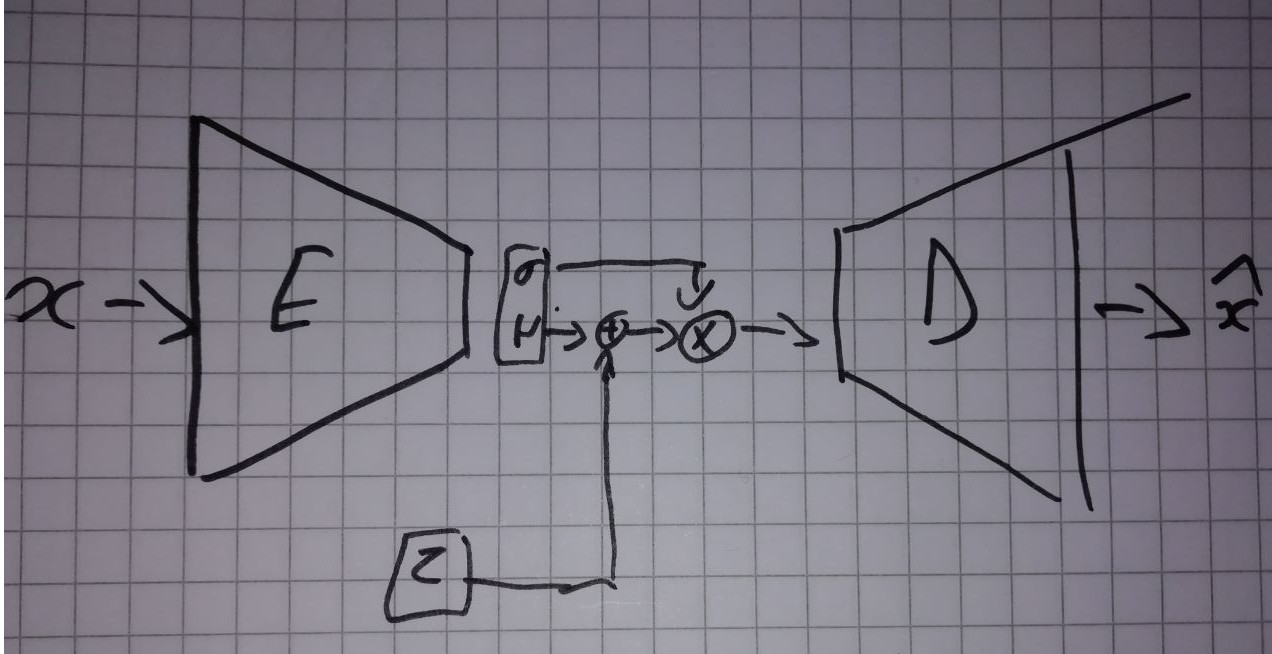
\includegraphics[height=\textheight/5,width=\textwidth*2/5]{chapter1/vae.jpg}
	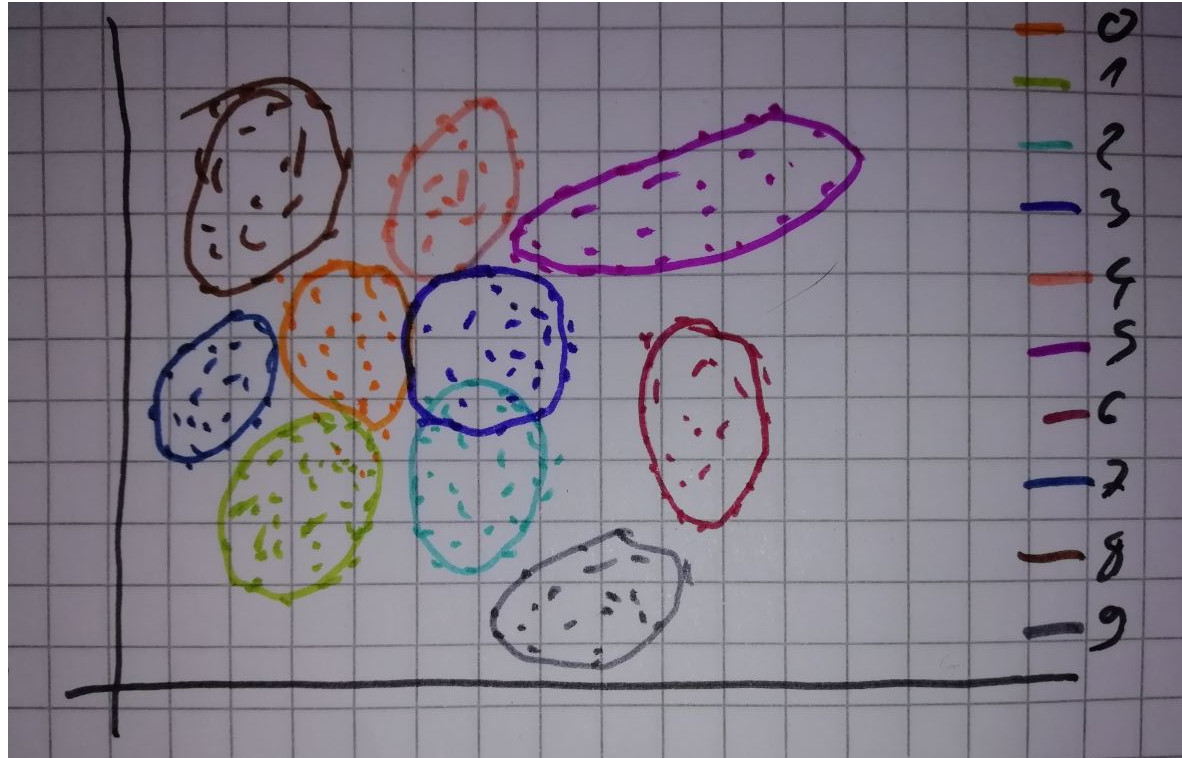
\includegraphics[height=\textheight/5,width=\textwidth*2/5]{chapter1/vae_latent.jpg}
	\caption[Variational auto-encoder]{Left: the Variational auto-encoder global architecture. Right: the latent space of a \ac{VAE} trained on the MNIST \cite{Lecun1998} dataset. We can observe a Gaussian component per class in the latent space,}
\end{figure}

Finally, generating a sample $\vx$ with the trained model can be done by sampling a random vector $\vz \sim  \mathcal{N}(0,1)$ and computing $\vx = \G(\vz)$.

\subsubsection{Normalizing flows}

Normalizing flow based techniques is a family of latent variable models that aim to tackle the marginalization problem by using the \textit{change of variable formula}

\begin{equation*}
	\pg{\vx} = \p{\vz} \Big|\det\Big(\frac{\partial\G(\vz)}{\partial{\vz^T}}\Big)\Big|^{-1}  = \p{\G^{-1}(\vx)} \Big|\det\Big(\frac{\partial\G^{-1}(\vx)}{\partial{\vx^T}}\Big)\Big|  \enspace ,
\end{equation*}
with $\vz \sim \p{\vz}$ a latent variable. This formulation has notable advantages such as explicitly allowing the computation of the exact inference. However, the model has to enforce some tough constraints: the input and output dimensions must be the same; $\G$ must be invertible; and computing the determinant of the Jacobian needs to be efficient and differentiable.

These constraints can be enforced through strong restrictions on the architecture of the model. By limiting the transformations to a set of invertible transformations with a tractable Jacobian determinant, the model remains invertible and the determinant of its Jacobian can be computed efficiently. 

Real-valued non-volume preserving (RealNVP) normalizing flows \cite{Dihn2016} uses affine coupling transformations, which transforms a variable by adding and scaling it by a non-linear transformation of itself, usually computed with deep neural networks. These transformations can be inverted by substracting and downscaling by the same transformed variables and their Jacobian is triangular, therefore computing its determinant can be done efficiently by computing the product of its diagonal terms.  \textit{Glow} \cite{Kingma2018} extended this set of transformations to $1\times1$ invertible convolutions as well as a variant of batch normalization that allows for more expressiveness in the model.

%$\vx$ into $\vy$ by partitioning it into $(\vx_1, \vx_2)$ and computing $\vy_1 = \vx_1; \vy_2 = \exp(s_\theta(\vx_1)) \odot \vx_2 + m_\theta(\vx_1)$, where $s_\theta$ and $m_\theta$ are arbitrary scaling and translation parametric functions. These transformations can be inverted as $\vx_1 = \vy_1; \vx_2 = \exp(-s_\theta(\vy_1)) \odot (\vx_2 - m_\theta(\vx_1))$ 


\section{Generative Adversarial Networks}

In this section, we will focus on the Generative Adversarial Networks \cite{Goodfellow2014} framework, their training process  and some of their variants, especially their conditional and domain-transfer variants.

We will then outline some limitations of this framework and propose a formulation of these limitations in the form of a trilemma between the intrinsic quality of the generated samples, their diversity and the quality of the conditioning of the model. With this tool, we propose a taxonomy of the recent \GAN approaches and identify trends in these approaches.


\subsection{The GAN framework}

In the same fashion as the generative models mentioned in \citesub{sub:deep_gen_modeling}, Generative Adversarial Networks (\ac{GANs})\cite{Goodfellow2014} aims to learn a parameterized mapping $\pg{\vx|\vz}$ between a simple distribution $\p{\vz}$ (usually normal or uniform) to the real data distribution $\p{\vx}$. However, instead of relying on the likelihood and trying to estimate the distribution through marginalization, it aims to minimize an estimation of a divergence between $\p{\vx}$ and the mapped distribution $\pg{\vx}$. 

Minimizing a divergence $\Div{\p{\vx}}{\pt{\vx}}$ allows for a parametric distribution $\pt{\vx}$ to converge to a target distribution $\p{\vx}$. When this divergence is both tractable (or estimable) and differentiable w.r.t the parameters $\theta$

In practice, divergences are usually intractable. To estimate such a divergence, \GANs rely on a second learned function that will act as an adversary: the discriminator $\D$.  The discriminator is a binary classifier that aims to predict the probability that a sample $x$ was sampled on the real distribution $\p{\vx}$ or was  generated from $z\sim\p{\vz}$ and is trained by minimizing the  binary cross-entropy. The objective of the generator $\G$ is then to fool the discriminator by maximizing the same binary cross-entropy. This training process is summed up as a mini-max game in \citeq{eq:GAN_problem} 

\begin{equation}
\label{eq:GAN_problem}
\arg\min_\G\max_\D\lgan = \arg\min_G\max_\D \esp{x\sim \p{\vx}} [\log \D(x)] +  \esp{z\sim\p{\vz}} [1 - \log \D(\G(z))] \enspace.
\end{equation}

\begin{figure}
	\centering
	
\includegraphics[height=\textheight/3,width=\textwidth]{foo.png}
	\caption{Generative Adversarial Networks framework}
\end{figure}

This mini-max game has, assuming infinite capacity for both $G$ and $D$, a global optimum for $\p{\vx} = \pg{\vx}$, which can be proved as follows: the minimum of $f(x) = a\log(x) + b\log(1-x)$ is $\frac{a}{a+b}$, the discriminator that maximizes the criterion for a fixed $\G$ is given by

\begin{equation*}
\label{eq:optimal_D}
\D^*_\G(x) = \frac{\p{\vx}}{\p{\vx} + \pg{\vx}} \enspace.
\end{equation*}

We can formulate a criterion $C(\G)$ by plugin this optimal discriminator in \citeq{eq:GAN_problem}

\begin{align*}
		C( \G) &= \max_\D\lgan(\D, \G) \nonumber\\
		& = \esp{x\sim \p{\vx}} \Big[\log \D^*(x)] +  \esp{z\sim P_z} \Big[1 - \log \D^*(\G(z))\Big] \nonumber = \esp{x\sim \p{\vx}} \Big[\log \D^*(x)\Big] +  \esp{{x}\sim \pg{\vx}} \Big[1 - \log \D^*(x)\Big] \nonumber \\
		& = \esp{x\sim \p{\vx}} \Big[\log \frac{\p{\vx}}{\p{\vx} + \pg{\vx}}\Big] +   \esp{{x}\sim \pg{\vx}} \Big[1 - \log  \frac{\pg{\vx}}{\p{\vx} + \pg{\vx}}\Big] \nonumber \enspace.
\end{align*}

Up to additive and multiplicative constants, the criterion  $C(\G)$ can be reformulated as

\begin{equation*}
		C(\G) = \DKL \Big(\p{\vx}\Big|\Big|\frac{\p{\vx}+\pg{\vx}}{2} \Big) + \DKL \Big(\pg{\vx} \Big|\Big| \frac{\p{\vx}+\pg{\vx}}{2} \Big) = 2\cdot\JSD \Big(\p{\vx}\Big|\Big|\pg{\vx} \Big) \enspace.
\end{equation*}

When the discriminator is trained to convergence, minimizing the criterion $C( \G) = \lgan(\D^*, \G)$ is equivalent to minimizing the Jensen-Shannon (\ac{JS}) divergence between $\p{\vx}$ and $\pg{\vx}$. The \GAN training process then consists in alternatively updating the discriminator and the generator via gradient ascent/descent. A summary of this process is presented in \citealg{alg:GAN_train}. 

\begin{algorithm}[!ht]
	\caption{The\GAN training algorithm}
	\label{alg:GAN_train}
	\begin{algorithmic}[H]
		\REQUIRE{$\trainsetX$ the real dataset, $G$ the generator model, and $D$ the discriminator model}
		\REPEAT
		\STATE sample a mini-batch $\lbrace x_i \rbrace_{i=1}^m$ from $\trainsetX$\;
		\STATE sample a mini-batch $\lbrace z_i \rbrace_{i=1}^m$ from $\p{\vz}$\;
		\STATE update $D$ by stochastic gradient ascent of
		\STATE \ \ \ \ $ \sum_{i=1}^{m}\log(D(x_i)) + \log(1-D(G(z_i)))$
		\STATE sample a a mini-batch $\lbrace z_j \rbrace_{j=1}^n$ from distribution $\p{\vz}$\;; 
		\STATE update $G$ by stochastic gradient descent of
		\STATE \ \ \ \ $ \sum_{j=1}^n \log(1-D(G(z_j)))$\;
		\UNTIL a stopping condition is met
		
	\end{algorithmic}
\end{algorithm}


\subsection{Conditional modeling with  \ac{CGAN}s}

While classical generative models such as \GANs try to unconditionally approximate the real-data distribution $\p{\vx}$, a conditional generative model aim to learn a model of the conditional distribution $\p{\vx|\vy}$, where $y \in \setY$ is a label of any kind.

Several extensions of the \GAN framework allow for conditional modeling. First introduced, Conditional \GANs (\ac{CGAN}s)\cite{Goodfellow2014}\cite{mirza17} simply adds the label $y$ as an input for both the discriminator and the generator. The new optimization problem that results from this change is summed-up in \citeq{eq:CGAN_problem} as follows

\begin{equation}
\label{eq:CGAN_problem}
		\arg\min_G\max_\D \lcgan = 	\arg\min_G\max_\D \esp{x,y\sim \p{\vx,\vy}} [\log \D(x, y)] +  \esp{y\sim \p{\vy} \\ z\sim\p{\vz}} [1 - \log \D(\G(y, z), y)]
\end{equation}

While this approach is trivially simple to implement, it relies entirely on the discriminator to use the label. Other approaches try to learn the conditional distribution by adding an explicit loss term to the optimization problem, such as Auxillary Classifier GAN (\ac{ACGAN}) \cite{Odena}. This approach aims to learn a conditional generative model with discrete labels by adding another output to the discriminator that acts as a classifier. The model is then trained by having both the generator and the discriminator minimize the categorical cross-entropy  between the real and predicted labels.

\subsection{Domain-transfer with \GANs}

Domain-transfer is the task of learning a mapping $\p{\vx|\vy}$ between two high-dimensional distributions $\p{\vx}$ and $\p{\vy}$ that maintains semantic information, for example changing the color palette of an image while keeping the same objects at the same position. \ac{CGAN}s already learn to model the conditional distribution $\p{\vx|\vy}$, and adding a way to enforce the consistency of the semantic information enables
domain-transfer.

Pix2Pix \cite{Isola2016} implemented this approach  explicitly by using paired samples $(x, y) \sim \p{\vx|\vy}$ forcing the generator to minimize the $\Lone$ reconstruction term between $x$ and $\G(y,z)$ (\citeq{ex:pix2pix}). 

\begin{equation}
\label{eq:pix2pix}
\arg\min_G\max_\D L_{p2p} =  \arg\min_G\max_\D \lcgan(\D, \G) +\lambda\esp{x\sim\p{\vx}\\y\sim\p{\vy}\\z\sim\p{\vz}} ||x - G(y, z)||_1
\end{equation}

However, this kind of approaches rely on paired data which can be very hard to obtain, especially in the case of natural images. When trying for example to transfer images of zebras to images of horses, you need a dataset of very similar zebras and horses in the exact same position for the $\Lone$ term to work.

This problem of paired data was solved by \ac{CycleGAN }\cite{Zhu} using cycle-consistency. Instead of training a single model $\G$ with reconstruction between $x$ and $\G(y,z)$, the CycleGAN approach train two domain-transfer models simultaneously: $\Gyx$ and $\Gxy$ that map samples from $\p{\vy}$ onto $\p{\vx}$ and $\p{\vx}$ onto $\p{\vy}$, respectively (\seefigure{fig:cyclegan}). This allows to compute the $\Lone$ reconstruction errors  $||x - \Gyx(\Gxy(x))||_1$ and $||y - \Gxy(\Gyx(y))||_1$, thus completely removing the need for paired data $(x,y)$. The training of the two models in done an adversarial setup, with two discriminators $\Dx$ and $\Dy$, and is summed up as an optimization problem in \citeq{eq:cyclegan}

\begin{figure}
	\centering
	
\includegraphics[height=\textheight/3,width=\textwidth]{foo.png}
	\caption{CycleGAN framework}
	\label{fig:cyclegan}
\end{figure}


\begin{align}
\label{eq:cyclegan}
\arg\min_{\Gxy, \Gyx}\max_{\Dx, \Dy} \lcycgan &=   \arg\min_{\Gxy, \Gyx}\max_{\Dx, \Dy} \lgan(\Dx, \Gyx) + \lgan(\Dy, \Gxy) \nonumber \\
& +\lambda \esp{x\sim\p{\vx}} ||x - \Gyx(\Gxy(x)||_1 + \lambda\esp{y\sim\p{\vy}} ||y - \Gxy(\Gyx(y)||_1
\end{align}

The \ac{CycleGAN} training process then consists in alternatively updating the two discriminator and the two generators via gradient ascent/descent. A summary of this process is presented in \citealg{alg:cyclegan_train}. 

\begin{algorithm}[]
	\begin{algorithmic}[H]
		\REQUIRE{$\setX$ and $\setY$ two unpaired datasets, $\Gxy$ and $\Gyx$ the mapping networks, $\Dx$ and $\Dy$ the discrimination models, $m$ the mini-batch size}
		\REPEAT
		\STATE sample a mini-batch $\lbrace x_i \rbrace_{i=1}^m$ from $\setX$\;
		\STATE sample a mini-batch $\lbrace y_i \rbrace_{i=1}^m$ from $\setY$\;
		\STATE update $\Dx$ by stochastic gradient descent of
		\STATE \ \ \ \ $ \sum_{i=1}^{m}(\Dx(x_i)-1)^2 + (\Dx(\Gyx(y_i)))^2$
		\STATE update $\Dy$ by stochastic gradient descent of
		\STATE \ \ \ \ $ \sum_{i=1}^{m}(\Dy(y_i)-1)^2 + (\Dy(\Gxy(x_i)))^2$
		\STATE sample a mini-batch $\lbrace x_i \rbrace_{i=1}^m$ from $X$\;
		\STATE sample a mini-batch $\lbrace y_i \rbrace_{i=1}^m$ from $Y$\;
		\STATE update $\Gxy$ by stochastic gradient descent of
		\STATE \ \ \ \ $ \sum_{i=1}^n (\Dy(\Gxy(x_i))-1)^2 + \lambda (||x_i - \Gyx(\Gxy(x_i))||_1$ \STATE \ \ \ \ \ \ \ \ $+||y_i -\Gxy(\Gyx(y_i))||_1)$\;
		\STATE update $\Gyx$ by stochastic gradient descent of
		\STATE \ \ \ \ $ \sum_{i=1}^n (\Dx(\Gyx(y_i))-1)^2+ \lambda (||x_i - \Gyx(\Gxy(x_i))||_1 $
		\STATE \ \ \ \ \ \ \ \ $+ ||y_i - \Gxy(\Gyx(y_i))||_1)$\;
		\UNTIL a stopping condition is met
	\end{algorithmic}
	\caption{CycleGAN training algorithm}
	\label{alg:cyclegan_train}
\end{algorithm}

\section{Limitations}

GANs have shown strong advantages over the classical generative modeling methods, such as generating sharper samples than \ac{VAE}s or taking significantly less time to train and to generate a sample than normalizing flows. However, they exhibit limitations: the instability of the training process; the lack diversity of the generated samples (\textit{mode-collapse}); and finally the problems due to conditioning. 

The instability of the \GAN training process has first been conjectured to be caused by the bad quality of the gradients obtained when $\G$ generates bad samples, which makes $\D$ strongly reject these samples and therefore saturating the loss. The first solution proposed \cite{Goodfellow2014} was to slightly change the generator's loss function from $\log(1-\D(\G(z)))$ to $-\log(\D(\G(z)))$, which helped considerably to avoid failures of the training process and was then widely used%TODO références.

 While this loss term converges to the same minimum as the original loss term, it however no longer correspond to a \ac{JSD}

\CR{
Image quality : Incremental enhancement through architecture, more data, ... 

Instability, catastrophic forgetting and the mode collapse problem

Trade-off image quality/diversity : Explanation through the loss term and distribution coverage

Black-box approach to conditioning, no tuning possible, no interpretability
}
\section{The GAN Zoo}

\subsection{A taxonomy of GANs}
Enorme nombre de variantes de GANs

Taxonomie des approches GANs (pour s'éviter une liste des différents GANs)

Schéma pour définir les grandes familles de GAN (évoquer les AmbientGAN / UNIR)

\subsection{Architecture variants}

\subsection{Divergence variants}
Table des loss alternatives (f-divergences + transport optimal)

\subsection{Task-specific losses}

\begin{figure}
	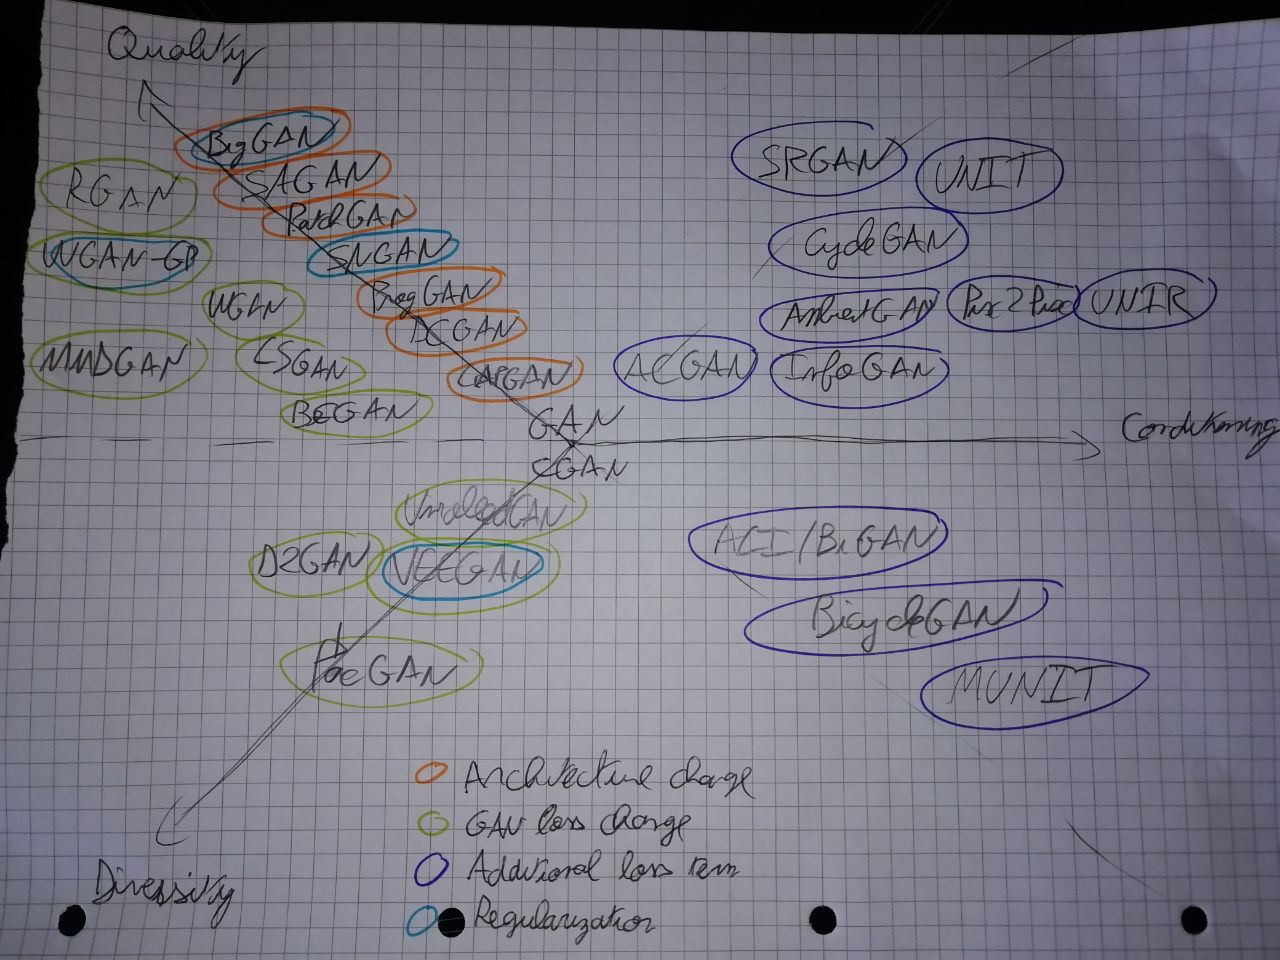
\includegraphics[width=\textwidth]{chapter1/trilemma.jpg}
	\caption{Classifications of some advances in GANs on the trilemma}
\end{figure}

\section{A note on the  evaluation of generative models}

No good adhoc methods

Image quality : Inception distance + Fréchet inception distance, advantages

Conditioning : Direct evaluation (pixel-wise), Classifier accuracy, Projections (PCA, t-SNE)

Limitations of those metrics : need a pre-trained model


